% RP^1 as lines through the origin in R^2, projected onto the tangent line y=1;
% the horizontal (cyan) line through the origin maps to the point at infinity.
% Source: book/tex/topology/constructions.tex (§ Real projective space).
\documentclass[border=2mm]{standalone}
\usepackage{tikz}
\usepackage{amssymb}
\usetikzlibrary{arrows.meta}
\begin{document}
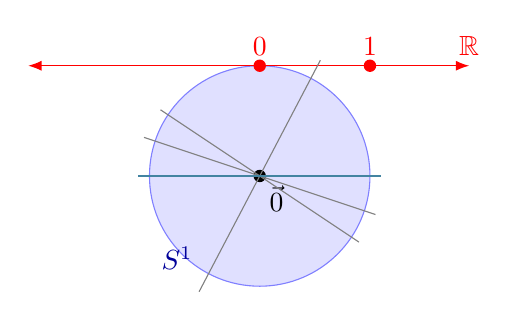
\begin{tikzpicture}[scale=1.4]
  \fill[blue!12] (0,0) circle (1);
  \draw[blue!50] (0,0) circle (1);
  \node[blue!60!black] at (-0.75,-0.75) {$S^1$};
  \fill (0,0) circle (1.6pt) node[below right] {$\vec 0$};
  % tangent line R at y = 1
  \draw[red,{Latex}-{Latex}] (-2.1,1) -- (1.9,1);
  \node[red,above] at (1.9,1) {$\mathbb{R}$};
  \fill[red] (0,1) circle (1.6pt) node[above] {$0$};
  \fill[red] (1,1) circle (1.6pt) node[above] {$1$};
  % a few lines through the origin
  \draw[gray] (-0.55,-1.05) -- (0.55,1.05);
  \draw[gray] (0.9,-0.6) -- (-0.9,0.6);
  \draw[gray] (1.05,-0.35) -- (-1.05,0.35);
  % the horizontal line -> point at infinity (parallel to R)
  \draw[cyan!60!black,thick] (-1.1,0) -- (1.1,0);
\end{tikzpicture}
\end{document}
